\documentclass[12pt]{book}
\usepackage[utf8]{inputenc}
\usepackage[margin=1.25in]{geometry}
% Packages for AMS math and symbols.
\usepackage{amsmath}
\usepackage{amssymb}
% Package and settings for theorems and proofs.
\usepackage{amsthm}
\newtheorem{theorem}{Theorem}
% Package for including figures.
\usepackage{graphicx}
% Adds a therefore symbol.
\def\therefore{\boldsymbol{\text{ }
\leavevmode
\lower0.4ex\hbox{$\cdot$}
\kern-.5em\raise0.7ex\hbox{$\cdot$}
\kern-0.55em\lower0.4ex\hbox{$\cdot$}
\thinspace\text{ }}}

% Shortcuts for common commands.
\renewcommand*{\vec}[1]{\mathbf{#1}}
\DeclareMathOperator{\sech}{sech}

% Package for hyperlinks.
\usepackage{hyperref}
\hypersetup{
    colorlinks=true,
    linkcolor=blue,
    %filecolor=magenta,      
    urlcolor=cyan,
}

% Define new environment for definitions
\newcounter{definition}[chapter]
\newenvironment{definition}[2]
    {\begin{flushleft}
    \hspace{10pt}
    \refstepcounter{definition}
    \textbf{#1}: {\emph{#2}}
    \end{flushleft}}

% Increase spacing in tables.
\setlength{\tabcolsep}{18pt}
\renewcommand{\arraystretch}{1.5}

%--------------------------------------------%
\title{UA PH 481 Review}
\author{Jalen Cates}
\date{\today}
%--------------------------------------------%

\begin{document}
%--------------------------------------------%
% Possible additions:
%   Chapter on bonding
%   Chapter on Phonons 1

\maketitle
\tableofcontents

% Output the crystal structure chapter.
%%%%%%%%%%%%%%%%%%%%%%%%%%%%%%%%%%%%%%%%%%%%%%%%%%%%%%%%%%%%%%%
\chapter{Crystal Structure in Solids}

Solids tend to arrange themselves into ordered, repeating structures. These can be conveniently described mathematically in the ways laid out in this chapter.



\begin{definition}
{lattice}{set of mathematical points to which the basis is attached}
\end{definition}

A lattice is defined by three translation vectors $\mathbf{a}_1, \mathbf{a}_2, \mathbf{a}_3$, such that integer $u_1, u_2, u_3$ movement along these are equivalent points:
\begin{equation} \label{eq:lattice-translation}
    \mathbf{r}' = \mathbf{r} + u_1\mathbf{a}_1 + u_2\mathbf{a}_2 + u_3\mathbf{a}_3
\end{equation}

\begin{definition}
{basis}{identical group (of atoms) that repeated infinitely to fill space}
\end{definition}
The position of the atom (or atoms) in the basis can be described by the position vector:
\begin{equation}
    \mathbf{r}_j = x_j\mathbf{a}_1 + y_j\mathbf{a}_2 + z_j\mathbf{a}_3 \;: \; 0 \leq x_j, y_j, z_j \leq 1 
\end{equation}

\begin{definition}
{primitive lattice}{Any two points from which the atomic arrangement looks the same satisfy \ref{eq:lattice-translation} with a suitable choice of the integers $u_i$}
\end{definition}
\begin{definition}
{primitive translation vectors}{Translation vectors $\mathbf{a}_i$ that satisfy the definition of the primitive lattice.}
\end{definition}

\begin{definition}
{crystal axes}{The set of primitive translation vectors that form the three adjacent edges of the primitive parallelepiped}
\end{definition}
It is often most convenient to use the crystal axes as the coordinate system in crystalline solids. The primitive translation vectors define the \emph{smallest volume} cell that can fill space with primitive translations. This volume is
\begin{equation}
    V_c = |\mathbf{a}_1 \cdot \mathbf{a}_2 \times \mathbf{a}_3|
\end{equation}

\begin{definition}
{primitive cell}{smallest-volume cell that will fill all space by primitive lattice translations. No basis contains fewer atoms than the primitive basis, and a primitive cell contains one lattice point.}
\end{definition}

\begin{definition}
{Wigner-Seitz Cell}
{primitive cell that can be constructed by the method:
\begin{enumerate}
    \item Draw vectors from a lattice point to its neighbors.
    \item Draw planes bisecting the vectors from step 1.
    \item Take the smallest volume enclosed by these planes.
\end{enumerate}
}
\end{definition}

\begin{figure}[h]
    \centering
    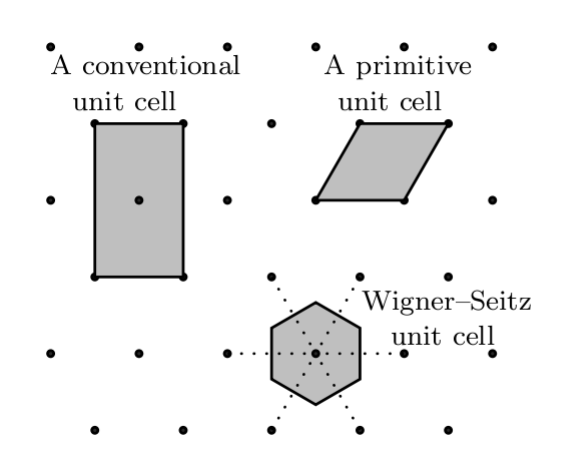
\includegraphics[width=0.5\textwidth]{./figures/wigner-seitz-ex.png}
    \caption{An example from lecture slides for Wigner-Seitz cell.}
    \label{fig:wigner-seitz-ex}
\end{figure}



%--------------------------------------------%
\section{Lattice Types}
A crystal lattice is repeated by translation vectors $\mathbf{T}$ and by various other symmetry operations. 
\begin{definition}
{Mirror Symmetry}{$(m)$ Reflection in a plane}
\end{definition}
\begin{definition}
{Inversion Symmetry}{$(\Bar{1})$ Reflection in a point}
\end{definition}
\begin{definition}
{N-fold Rotational Symmetries}{$(C_n)$ Rotations of $2\pi/n$ about point}
\end{definition}

\begin{theorem}
The only allowed rotational symmetries in a discrete lattice are 2-fold, 3-fold, 4-fold, and 6-fold.
\end{theorem}
Although molecules can have any rotational symmetries, there is a theorem about the allowed rotational symmetries in a lattice. We had to prove this for a two-dimensional lattice on our homework, but a helpful webpage \href{http://www.xtal.iqfr.csic.es/Cristalografia/parte_03_1_1-en.html}{here} explains it well.

\begin{definition}
{Bravais Lattice}{common phrase for distinct lattice types. There are 5 in two dimensions and 14 in three dimensions.}
\end{definition}

%--------------------------------------------%
\subsubsection{Two-Dimensional Lattice Types}
\begin{table}[h]
    \centering
    \begin{tabular}{l|c|c}
        \textbf{Name} & \textbf{Distances} & \textbf{Angles} \\
        \hline
        Oblique      & $|a_1|\neq |a_2|$ & \\
        Square       & $|a_1|=|a_2|$     & $\phi=\pi/2$ \\
        Rectangular  & $|a_1|\neq |a_2|$ & $\phi=\pi/2$ \\
        Hexagonal    & $|a_1|=|a_2|$     & $\phi=2\pi/3$ \\
        Centered Rectangular  & $|a_1|\neq |a_2|$ & $\phi=\pi/2$
    \end{tabular}
    \caption{Bravais Lattice types in two dimensions.}
    \label{tab:2d-bravais}
\end{table}
A centered rectangular lattice is a rectangular lattice with a lattice point in the center of it.

%--------------------------------------------%
\subsubsection{Three-Dimensional Lattice Types}
\begin{table}[h]
    \centering
    \begin{tabular}{l|c|c|c}
        \textbf{Name} & \textbf{Lattices} & \textbf{Distances} & \textbf{Angles} \\
        \hline
        Triclinic    & 1 & $|a_1|\neq |a_2|\neq |a_3|$ & $\alpha\neq\beta\neq\gamma$ \\
        Monoclinic   & 2 & $|a_1|\neq |a_2|\neq |a_3|$ & $\alpha=\gamma=\pi/2\neq\beta$ \\
        Orthorhombic & 4 & $|a_1|\neq |a_2|\neq |a_3|$ & $\alpha=\beta=\gamma=\pi/2$ \\
        Tetragonal   & 2 & $|a_1|=|a_2|\neq |a_3|$     & $\alpha=\beta=\gamma=\pi/2$ \\
        Cubic        & 3 & $|a_1|=|a_2|=|a_3|$         & $\alpha=\beta=\gamma=\pi/2$ \\
        Trigonal     & 1 & $|a_1|=|a_2|=|a_3|$         & $\alpha=\beta=\gamma<2\pi/3,\neq\pi/2$ \\
        Hexagonal    & 1 & $|a_1|=|a_2|\neq |a_3|$     & $\alpha=\beta=\pi/2,\; \gamma=2\pi/3$ \\
    \end{tabular}
    \caption{Bravais Lattice types in three dimensions.}
    \label{tab:3d-bravais}
\end{table}


%--------------------------------------------%
\subsection{Cubic Lattices}
The three cubic lattices are simple cubic (sc), body-centered cubic (bcc), and face-centered cubic (fcc). Some useful properties are summarized in the table below.

\begin{table}[h!]
    \centering
    \begin{tabular}{l|c|c|c}
        \textbf{Property} & \textbf{Simple} & \textbf{Body-centered} & \textbf{Face-centered} \\
        \hline
        Lattice points per cell & 1 & 2 & 4 \\
        Volume of primitive cell & $a^3$ & $a^3/2$ & $a^3/4$ \\
        Number of nearest neighbors & 6 & 8 & 12 \\
        Packing fraction &  $\frac{1}{6}\pi$ & $\frac{\sqrt{3}}{8}\pi$ & $\frac{\sqrt{2}}{6}\pi$
    \end{tabular}
    \caption{Some properties of cubic lattices.}
    \label{tab:cubic-properties}
\end{table}

Cubic systems have the highest number of symmetries. They are:
\begin{enumerate}
    \item Inversion symmetry for center of cell $(C_i)$
    \item Six mirror planes $(C_s)$
    \item Three 4-fold symmetry axes $(C_4)$
    \item Four 3-fold axes $(C_3)$
    \item Four 2-fold axes $(C_2)$
\end{enumerate}
%--------------------------------------------%
\subsubsection{Primitive Cubic Lattice}
The primitive cell of the \emph{simple cubic} cell is itself, with lattice vectors:
\begin{equation*}
    \mathbf{a}_1 = a \hat{\mathbf{x}} \quad \mathbf{a}_2 = a \hat{\mathbf{y}} \quad \mathbf{a}_3 = a \hat{\mathbf{z}}
\end{equation*}

%--------------------------------------------%
\subsubsection{Body-Centered Cubic Lattice}
Examples include alkali metals, Ba, Nb, W, and bcc Cr or Fe. The Wigner-Seitz cell of the \emph{body-centered cubic} cell is a \emph{truncated octahedron}, with lattice vectors:
\begin{align*}
    \mathbf{a}_1 & = \frac{1}{2} a (\hat{\mathbf{x}} + \hat{\mathbf{y}} - \hat{\mathbf{z}}) \\
    \mathbf{a}_2 & = \frac{1}{2} a (-\hat{\mathbf{x}} + \hat{\mathbf{y}} + \hat{\mathbf{z}}) \\
    \mathbf{a}_3 & = \frac{1}{2} a (\hat{\mathbf{x}} - \hat{\mathbf{y}} + \hat{\mathbf{z}}) 
\end{align*}

%--------------------------------------------%
\subsubsection{Face-Centered Cubic Lattice}
Examples include Cu, Ag, Au, Ni, Pd, Pt, and Al. The Wigner-Seitz cell of the \emph{face-centered cubic} cell is a \emph{rhombic dodecahedron}, with lattice vectors:
\begin{align*}
    \mathbf{a}_1 & = \frac{1}{2} a (\hat{\mathbf{x}} + \hat{\mathbf{y}}) \\
    \mathbf{a}_2 & = \frac{1}{2} a (\hat{\mathbf{y}} + \hat{\mathbf{z}}) \\
    \mathbf{a}_3 & = \frac{1}{2} a (\hat{\mathbf{x}} + \hat{\mathbf{z}}) 
\end{align*}



%--------------------------------------------%
\section{Index System for Crystal Planes}
Crystal planes can be defined by their intercepts
\begin{equation*}
    S_1 = m_1 \mathbf{a} \quad S_2 = m_2 \mathbf{b} \quad S_3 = m_3 \mathbf{c}
\end{equation*}

\subsubsection{Miller index}
The common system for indexing planes in a lattice. They are found by the method below.
\begin{enumerate}
    \item Calculate the reciprocal values $\frac{1}{m_1}$, $\frac{1}{m_2}$, $\frac{1}{m_3}$
    \item Multiply those values with the smallest integer $p$, which turns the values into integers $h=\frac{p}{m_1}$, $k=\frac{p}{m_2}$, and $l=\frac{p}{m_3}$
    \item The index of the plane is $(hkl)$\footnote{Negative intercepts are denoted with a bar above the index.}
\end{enumerate}

The normal vector of a set of planes is
\begin{equation*}
    \mathbf{n} = h \, \mathbf{a} + k \, \mathbf{b} + l \, \mathbf{c} \equiv [hkl]
\end{equation*}



%--------------------------------------------%
\section{Atomic Packing Factor}
\begin{definition}
{Atomic Packing Factor (APF)}{Fraction of cell volume that is occupied by atoms}
\end{definition}
\begin{equation}
    APF = \frac{N_{atoms}V_{atoms}}{V_{cell}}
\end{equation}

If one tries to construct the structure that is \emph{close-packed}, there are two options with $APF=0.74$. Stacking layers in the sequence $ABAB...$ leads to \emph{hexagonal close-packed} structure, and stacking in the sequence $ABCABC...$ gives the fcc structure.

\vspace{10pt}
\textbf{Note:} This chapter also included $NaCl$, $CsCl$, and Diamond structures as examples of simple lattices.
%--------------------------------------------%
% Possible additions:
%   Examples like NaCl and CsCl
%   Figures


% Output the chapter on reciprocal lattice.
%%%%%%%%%%%%%%%%%%%%%%%%%%%%%%%%%%%%%%%%%%%%%%%%%%%%%%%%%%%%%%%
\chapter{Wave Diffraction and Reciprocal Lattice}
The familiar condition for constructive interference in scattering is the \textbf{Bragg law}:
\begin{equation}
    2\, d\, \sin{\theta} = n\, \lambda, \quad \lambda \leq 2d
\end{equation}
We need a more sophisticated way to look at scattering though. Direct imaging of a lattice has a limit to its resolution, so indirect imaging is necessary.



%--------------------------------------------%
\section{Theory of Scattering}
\emph{Elastic} scattering is considered in depth in this section. One should recall basic properties of waves, including diffraction, coherence, and \emph{Huygen's Principle.}
\begin{definition}
{Huygen's Principle}{Every point on a wavefront is itself a source of spherical waves}
\end{definition}
\begin{definition}
{Coherent scattering}{Assume a fixed phase between primary and emitted waves.\footnote{Valid approximation for x-rays and neutrons.}}
\end{definition}

A plane wave with initial amplitude $A_0$, frequency $\omega_0$, and wave vector $\mathbf{k}_0$ at scattering center $P$ is
\begin{equation*}
    A_P(\mathbf{r}, t) = A_0 e^{i(\mathbf{k}_0\cdot(\mathbf{R}+\mathbf{r})-\omega_0 t)}
\end{equation*}
Where $\mathbf{R}$ points to the origin in the crystal, and $\mathbf{r}$ points from the origin to $P$. The detected wave at $B$, which is $\mathbf{R}'$ relative to the origin, can be written as
\begin{equation*}
    A_B(\mathbf{r}, t) = A_P(\mathbf{r}, t) \rho(\mathbf{r}, t) \frac{e^{ik|\mathbf{R}'-\mathbf{r}|}}{|\mathbf{R}'-\mathbf{r}|}
\end{equation*}
The total observed amplitude at time $t$ is 
\begin{equation*}
    A_B(t) = \frac{A_0}{R'} e^{i(\mathbf{k}_0\cdot\mathbf{R}+\mathbf{k}\cdot\mathbf{R}')}e^{-i\omega_o t}\int \rho(\mathbf{r}, t)e^{i(\mathbf{k}_0-\mathbf{k})\cdot \mathbf{r}} d\mathbf{r}
\end{equation*}

The \emph{intensity of scattered waves} for \emph{scattering vector} $\mathbf{K}=\mathbf{k}-\mathbf{k}_0$ with \emph{scattering amplitude} $\mathcal{A}(\mathbf{K})$ is
\begin{equation*}
    I(\mathbf{K}) \propto |A_B(t)|^2 \propto \bigg|\int \rho(\mathbf{r})e^{-i(\mathbf{K})\cdot \mathbf{r}} d\mathbf{r}\bigg|^2
\end{equation*}


%--------------------------------------------%
\subsection{Fourier Transform of Lattice}
The \emph{Fourier Transform} gives a powerful way to relate the \emph{scattering amplitude} and \emph{scattering density}.

\begin{equation}
    \mathcal{A}(\mathbf{K}) = \int \rho(\mathbf{r})e^{-i(\mathbf{K})\cdot \mathbf{r}} d\mathbf{r} \iff \rho(\mathbf{r}) = \frac{1}{(2\pi)^3} \int \mathcal{A}(\mathbf{K}) e^{i(\mathbf{K})\cdot \mathbf{r}} d\mathbf{K}
\end{equation}

This leads to the relation for discrete lattice points with set of vectors $\mathbf{G}$:
\begin{equation}
    \rho (\mathbf{r}) = \sum_\mathbf{G} \rho_\mathbf{G} e^{i\mathbf{G}\cdot \mathbf{r}}
\end{equation}
We need to construct 
\begin{equation}
    \mathbf{G} = h \,\mathbf{g}_1 + k \,\mathbf{g}_2 + l \,\mathbf{g}_3
\end{equation}
such that
\begin{equation}
    \mathbf{g}_i \cdot \mathbf{a}_j = 2\pi \delta_{ij}
\end{equation}

The \emph{reciprocal basis} $\mathbf{G}$, fulfills the condition above. The vectors have dimensions of inverse length, and these are in \emph{reciprocal space, k-space, or momentum space}. The standard basis is constructed by
\begin{align*}
    \mathbf{g}_1 & = 2\pi \frac{\mathbf{a}_2\times\mathbf{a}_3}{\mathbf{a}_1\cdot(\mathbf{a}_2\times\mathbf{a}_3)} \\
    \mathbf{g}_2 & = 2\pi \frac{\mathbf{a}_3\times\mathbf{a}_1}{\mathbf{a}_1\cdot(\mathbf{a}_2\times\mathbf{a}_3)} \\
    \mathbf{g}_3 & = 2\pi \frac{\mathbf{a}_1\times\mathbf{a}_2}{\mathbf{a}_1\cdot(\mathbf{a}_2\times\mathbf{a}_3)} \\
\end{align*}

\begin{definition}
{1st Brillouin Zone}{Wigner-Seitz cell in reciprocal space}
\end{definition}
\begin{definition}
{Higher-order Brillouin Zones}{Wigner-Seitz cell construction for further neighbors in reciprocal space}
\end{definition}



%--------------------------------------------%
\section{Scattering Condition}
The last section gives us
\begin{equation*}
    I(\mathbf{K}) \propto |A_B(t)|^2 \propto \bigg|\sum_\mathbf{G} \rho_\mathbf{G} \int e^{i(\mathbf{G}-\mathbf{K})\cdot \mathbf{r}} d\mathbf{r}\bigg|^2
\end{equation*}

This relation implies the only contribution comes when $\mathbf{G}-\mathbf{K}=0$.


%--------------------------------------------%
\subsection{Laue Condition}
\begin{definition}
{Laue Condition}{$(\mathbf{G}=\mathbf{K})$ gives the cases when scattered beams are seen.}
\end{definition}
When the \emph{Laue Condition} is met, the intensity of diffracted beams is
\begin{equation*}
    I(\mathbf{K}=\mathbf{G}) \propto |A_B(t)|^2 \propto |\rho_\mathbf{G}|^2 V^2
\end{equation*}

\textbf{Sophisticated Bragg Condition:} Kittel manipulates the condition $\mathbf{G}-\mathbf{K}=0$ to get
\begin{equation} \label{eq:bragg2}
    2 \mathbf{k}\cdot \mathbf{G} = G^2
\end{equation}
which he says is the common expression for the condition for diffraction. Relate this to Bragg condition by noting the distance between parallel planes is $d(hkl)=2\pi/|\mathbf{G}|$.

%--------------------------------------------%
\subsubsection{Laue Equations}
\textit{The Laue Equations} give a geometric condition that allows construction of an \textbf{Ewald Sphere}. They are
\begin{equation*}
    \mathbf{a}_1 \cdot \mathbf{K} = 2\pi v_1; \quad \mathbf{a}_2 \cdot \mathbf{K} = 2\pi v_2; \quad \mathbf{a}_3 \cdot \mathbf{K} = 2\pi v_3
\end{equation*}

%--------------------------------------------%
\subsubsection{Brillouin Zones}
The First Brillouin Zone is the Wigner-Seitz cell in reciprocal space. We can see a nice illustration of the diffraction condition if we divide \ref{eq:bragg2} by 4 on both sides.

\begin{equation} 
    \mathbf{k}\cdot (\mathbf{G}/2) = (G/2)^2
\end{equation}

In general, wave propagation is discussed in terms of the Brillouin Zone. \emph{Any wavevector starting at the origin and terminating on the surface of the Brillouin Zone will be diffracted.}



%--------------------------------------------%
\section{Reciprocal Lattices of Common Systems}
It is a good idea to know the cubic lattices very well. These are most likely to be used in calculations for class.

\subsection{Simple-Cubic Reciprocal Lattice}
The primitive cell of the \emph{simple cubic} cell is itself, with lattice vectors:
\begin{equation*}
    \mathbf{a}_1 = a \hat{\mathbf{x}} \quad \mathbf{a}_2 = a \hat{\mathbf{y}} \quad \mathbf{a}_3 = a \hat{\mathbf{z}}
\end{equation*}

The reciprocal lattice vectors are the set
\begin{equation*}
    \mathbf{g}_1 = (2\pi/a) \hat{\mathbf{x}} \quad \mathbf{g}_2 = (2\pi/a) \hat{\mathbf{y}} \quad \mathbf{g}_3 = (2\pi/a) \hat{\mathbf{z}}
\end{equation*}

The \textbf{reciprocal lattice} of the simple-cubic lattice is \textit{another} simple-cubic lattice. This also implies that the first Brillouin zone is also the simple-cubic lattice in k-space.
%--------------------------------------------%
% Possible additions:
%   Ewald Sphere
%   Structure Factor
%   Laue Method and Rotating Crystal
%   Reciprocal lattices


%

%%%%%%%%%%%%%%%%%%%%%%%%%%%%%%%%%%%%%%%%%%%%%%%%%%%%
\end{document}
